\documentclass[12pt]{report}

\usepackage[utf8]{inputenc}



\usepackage[a4paper,  total={6in, 8in}]{geometry}



\usepackage{ragged2e} %--For text alignment

\newenvironment{frontmatter}{}{\maketitle}

\usepackage{longtable}

\usepackage{graphicx}
\usepackage{rotating}
\usepackage{amssymb,amsmath}
%% The lineno packages adds line numbers. Start line numbering with
%% \begin{linenumbers}, end it with \end{linenumbers}. Or switch it on
%% for the whole article with \linenumbers after \end{frontmatter}.
%\usepackage{lineno}
\newtheorem{theorem}{Definition}
\usepackage{subfigure}
\usepackage{lscape}
%\usepackage{datetime}

%\usepackage{fancyhdr}
% 
%\pagestyle{fancy}
%\fancyhf{}
%\rhead{Put your tit}
%\lhead{Title}
%\rfoot{Page \thepage}


\begin{document}

\begin{titlepage}
    \begin{center}
        \vspace*{1cm}
        \Huge
        \textbf{Report	 Title}
        
        \vspace{0.5cm}
        \LARGE
        Report Subtitle (if any)
        
        \vspace{1.5cm}
        
        \textbf{Author Name}
         
         University Roll No.105XXXXXXXX          
        
        \vfill
        
        A technical report presented in partial fulfillment for the degree of
        Masters of Technology in Computer Science \& Engineering
        
        \vspace{0.8cm}
        
        
\includegraphics[width=0.4\textwidth]{buie_logo.jpg}
        
        Department Computer Science \& Engineering\\
        Bankura Unnayani Institute of Engineering\\
        Bankura - 722 146, West Bengal, India\\
       
       {November,}{\hspace*{0.5cm}}{2016}
       %\date{\displaydate{date}}
        
    \end{center}
\end{titlepage}
\newpage

\pagenumbering{gobble} 




\newpage
\begin{center}
        \vspace*{1cm}
         \LARGE
        \textbf{Certificate}
        
        \vspace{0.8cm}
 \justify      
		This is certified that the work contained in this report entitled, TITLE, by NAME, has been carried out under the supervision of the undersign and this work has not been submitted elsewhere for any other degree.       
        
        \vspace{2.0cm}
        
  \begin{flushleft}
  %\small
(Signature of the Supervisor)\\
Mr. X Y, Assistant Professor\\
Department of CSE\\
Bankura Unnayani Institute of Engineering\\
Bankura, West Bengal

\vspace{1.5cm}


(Signature of the HoD)\\
Mr. X Y, Associate Professor\\
 Department of CSE\\
Bankura Unnayani Institute of Engineering\\
Bankura, West Bengal


\end{flushleft}        
      
 
        
        \vfill
        
       
        
        
        
    \end{center}

    


\newpage
\vspace*{1cm}
\begin{center}
\LARGE
\textbf{Abstract}
\end{center}
\normalsize
\justify
 your abstract begins here.........\\
 Write your abstract in maximum 200-300 words.
 
 \vspace*{1cm}
 \smallskip
\noindent \textbf{Keywords.} list of keywords.
 Put atleast 6-8 keywords of your thesis work separated by coma(,)
 

\newpage
%\addcontentsline{toc}{chapter}{*}
\tableofcontents



\listoffigures


\newpage

\listoftables

\newpage
%\setcounter{page}{1}
\pagenumbering{arabic}
\chapter{Introduction}
%\justify
This  is  the  second  paragraph. Hello, here is some text without 
a meaning.  This text should show what 
a printed text will look like at this place.  If you read this text, 
you will get no information.  Really?  Is there no information?  Is there 
a difference between this text and some nonsense like not at all!  A 
blind text like this gives you information about the selected font, how 
the letters are written and an impression of the look.  This text should
contain all letters of the alphabet and it should be written in of the
original language.There is no need for special content, but the length of
words should match the language.

\newpage

\chapter{Background Theory}

{\bf Mathematical Equations}\\

You can write your mathematical equation as like in Eq.(\ref{eq:1}).

\begin{equation}
\label{eq:1}
X_{i}^{2}+Y_{j}^{2}=Z_{k}^{2}
\end{equation}


\newpage

\chapter{Review}

\newpage
\chapter{Materials \& Methods}
\section{Example of Table}



\begin{table}[h]
\centering
\caption{Table to test captions and labels}
\label{table:1}
\begin{tabular}{ |c| c| c| }
\hline
 cell1 & cell2 & cell3 \\ 
 \hline
 cell4 & cell5 & cell6 \\ 
 \hline 
 cell7 & cell8 & cell9   \\ 
 \hline
\end{tabular}

\end{table}




The table \ref{table:2} is an example of referenced \LaTeX elements.
\begin{sidewaystable}[h]
%\begin{table}[]
\centering
\caption{Table to test captions and labels}
\label{table:2}
\begin{tabular}{ |c| c| c| }
\hline
 cell1 & cell2 & cell3 \\ 
 \hline
 cell4 & cell5 & cell6 \\ 
 \hline 
 cell7 & cell8 & cell9   \\ 
 \hline
\end{tabular}

%\end{table}
\end{sidewaystable}




{\bf Multi-page tables}\\

If you have to insert a very long table, which takes up two or more pages in your document, use the longtable package. First, add to the preamble the line

\begin{verbatim}
\usepackage{longtable}
\end{verbatim}


\begin{longtable}[c]{| c | c |}
 \caption{Long table caption.\label{long}}\\
 
 \hline
 \multicolumn{2}{| c |}{Begin of Table}\\
 \hline
 Something & something else\\
 \hline
 \endfirsthead
 
 \hline
 \multicolumn{2}{|c|}{Continuation of Table \ref{long}}\\
 \hline
 Something & something else\\
 \hline
 \endhead
 
 \hline
 \endfoot
 
 \hline
 \multicolumn{2}{| c |}{End of Table}\\
 \hline\hline
 \endlastfoot
 
 Lots of lines & like this\\
 Lots of lines & like this\\
 Lots of lines & like this\\
 Lots of lines & like this\\
 Lots of lines & like this\\
 Lots of lines & like this\\
 Lots of lines & like this\\
 Lots of lines & like this\\
 ...
 Lots of lines & like this\\
 \end{longtable}

%The table \ref{table:3} is an example of referenced \LaTeX elements in landscape.
%
%\begin{landscape}
%
%\begin{table}[bth]
%\begin{center}
%\caption{Table to test captions and labels}
%\label{table:3}
%\begin{tabular}{ |c| c| c| }
%\hline
% cell1 & cell2 & cell3 \\ 
% \hline
% cell4 & cell5 & cell6 \\ 
% \hline 
% cell7 & cell8 & cell9   \\ 
% \hline
%\end{tabular}
%
%\end{center}
%\end{table}
%
%\end{landscape}

\newpage

\chapter{Results \& Discussion}

The graph is given in Fig.~\ref{fig:logo}.

\begin{figure}[!bth]
\center
\label{fig:logo}
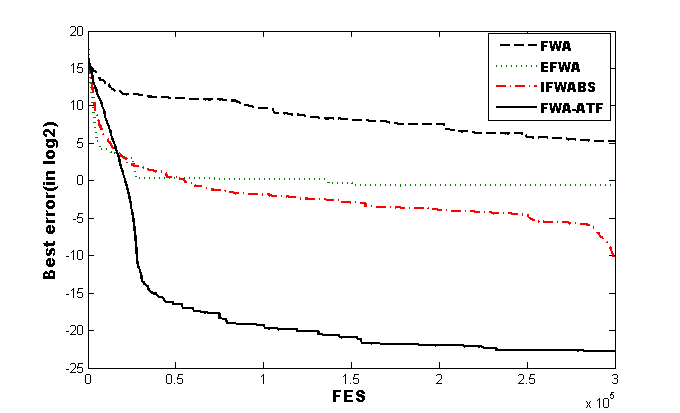
\includegraphics[scale=0.6]{f1.png}
\caption{Graph}
\end{figure}


If you need to place multiple images all together, use this...


\begin{figure}[!h]
  \centering
   \begin{tabular}{l l l}
  \subfigure[\label{db1mri1}]{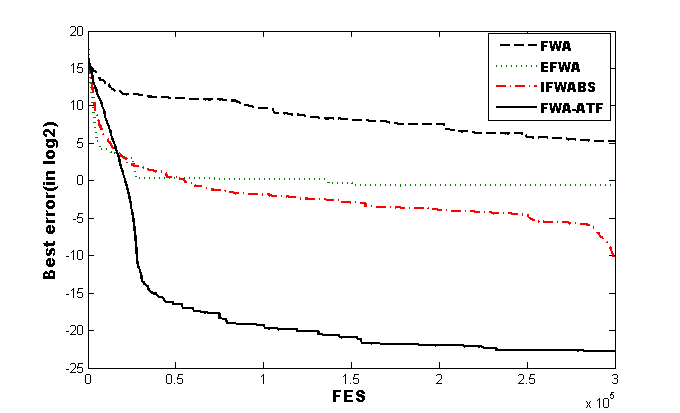
\includegraphics[width=1.4in,height=1.2in]{f1.png}}   &
   
  \subfigure[\label{db1mri2}]{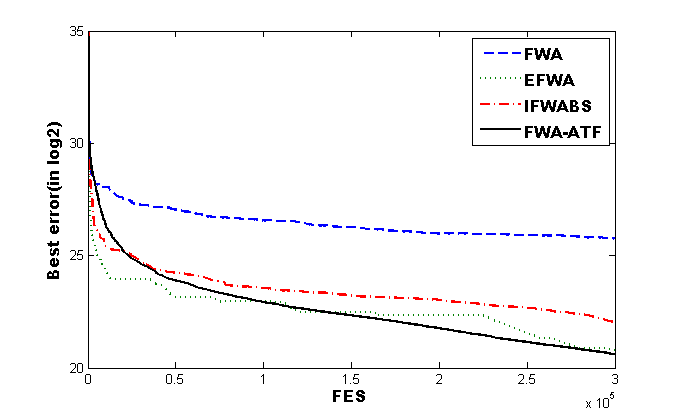
\includegraphics[width=1.4in,height=1.2in]{f2.png}}   &
 
  \subfigure[]{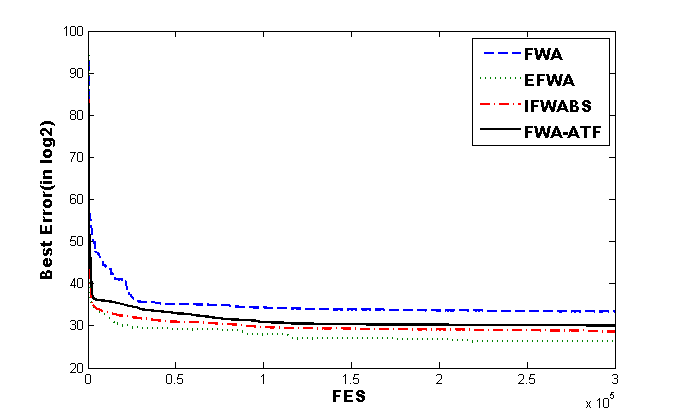
\includegraphics[width=1.4in,height=1.2in]{f3.png}}  \\

  \subfigure[]{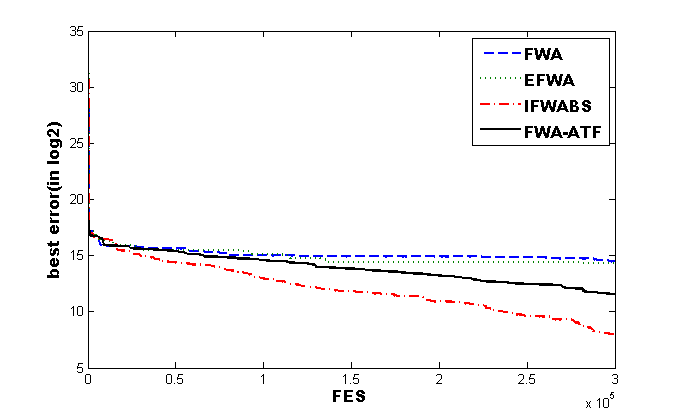
\includegraphics[width=1.4in,height=1.2in]{f4.png}}   &
 
  \subfigure[]{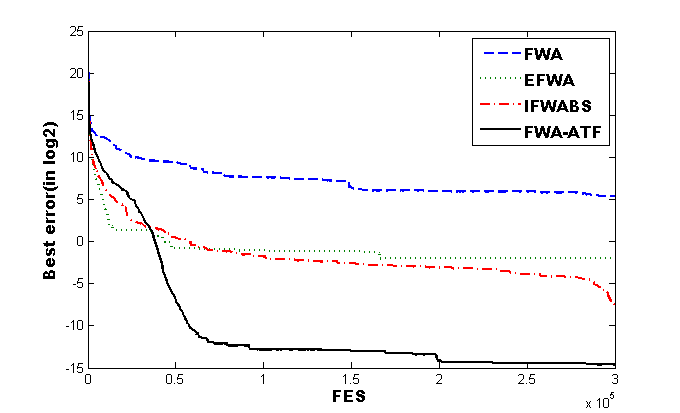
\includegraphics[width=1.4in,height=1.2in]{f5.png}}   &

  \subfigure[]{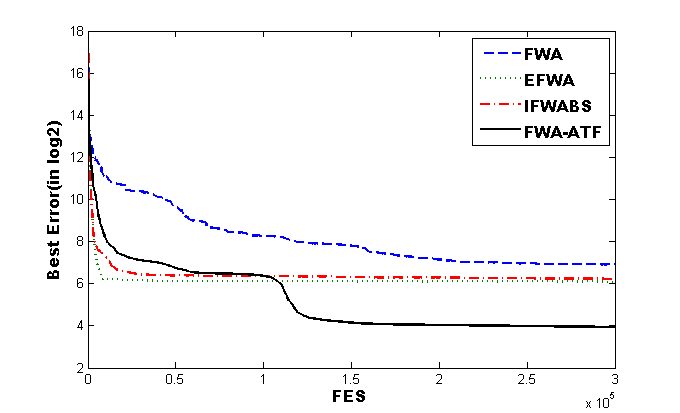
\includegraphics[width=1.4in,height=1.2in]{f6.png}}   \\
   \end{tabular}   
  \caption{put the caption}.
 \label{fig:db1}
\end{figure}



\newpage

\chapter{Conclusions}

\newpage

\chapter{Future Works}
Here you can outline the future scopes of your work..........
\newpage

\chapter*{List of Publications}
\begin{enumerate}
\item Author's name, Title, Conference, date, place, year, pp.~xx-xx.
\item Author's name, Title, Journal, Vol~X, No.~X, Year, pp.~xx-xx.
\end{enumerate}
\newpage
\begin{thebibliography}{00}
\bibitem{Derrac}
J. Derrac, S. Garcia, D. Molina and  F. Herrera, A practical tutorial on the use of nonparametric statistical tests as a methodology for comparing evolutionary and swarm intelligence algorithms. Swarm and Evolutionary Computation, 1(2011), 3--18
\end{thebibliography}


\end{document}
